\documentclass{article} % For LaTeX2e
\usepackage{hyperref}
\usepackage{url}
\usepackage[utf8]{inputenc}
\usepackage{amsmath}
\usepackage[numbers,sort]{natbib}
\usepackage{graphicx}
\usepackage[export]{adjustbox}
\usepackage{footmisc}
\usepackage[section]{placeins}
\usepackage{hyperref}
\DeclareGraphicsExtensions{.pdf,.png,.jpg,.eps}

\newlength\tindent
\setlength{\tindent}{\parindent}
\setlength{\parindent}{0pt}
\renewcommand{\indent}{\hspace*{\tindent}}


\author{
Gabriel C-Parent\\
}


\newcommand{\fix}{\marginpar{FIX}}
\newcommand{\new}{\marginpar{NEW}}

\begin{document}


\title{IFT6751: Homework 3}
      
\maketitle
\section{Introduction}

In this homework, an Elastic Net algorithm is used to solve the traveling salesperson problem (TSP). Using %\href{TSPLIB 

 different approaches to solve the capacitated vehicle routing problem (CVRP) were designed. The first one is a genetic algorithm using specialized crossover and mutation operators whereas the the second one uses the Tabu Search to control local search with the $\lambda$-interchange neighbourhood.\newline

Two greedy local search methods are used within both methods to improve the results such as the 2-opt descent and  and the $\lambda$-interchange descent.\newline

Another method based on the Clarke \& Wright savings is also used to initialize solutions for both metaheuristics.\newline




A description of all the optimization methods along with special implementation details is given.
Some experimental results are then compared based on running time, implementation complexity and results quality.\newline

Finally, a user guide is given in the supplementary section \ref{user_guide}.



\newpage
\section{Local Search Methods}
\label{local_search}

\subsection{2-opt descent}
\label{local_tsp}

First, a simple and fast optimization method for the TSP was needed to improve the path of each routes.\newline

The local search method used to optimize individual routes is the steepest improvement method as described in \citep{steepest_improvement}.
Basically, it is an implementation of steepest descent implementation using the well known 2-opt operator.\newline

At each iteration, the best possible 2-opt is chosen, according to the reduction in total distance, until there isn't any possible improvement. The complexity of the procedure $O(n^{2})$ on the number of edges in the route.\newline

Although it might seem slow, usually the number of edges is quite small and the time spent optimizing routes is negligible.\newline


%------------------------------------------------------------------------------
\newpage
\section{Experimental Results}
\label{exp_results}

\begin{figure}[!htb]
\begin{center}
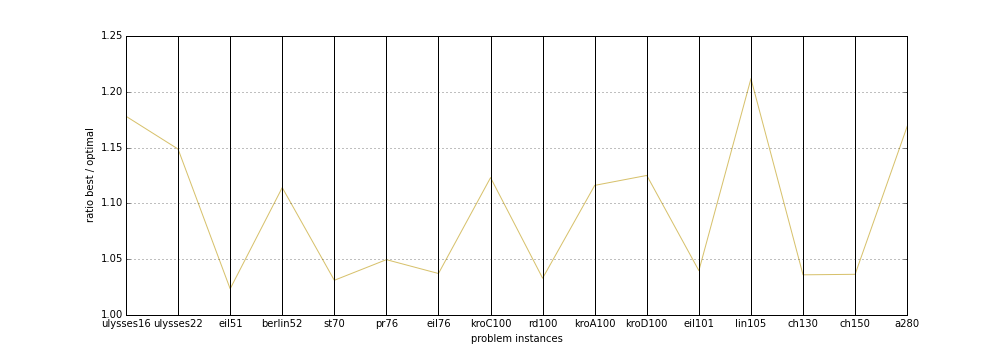
\includegraphics[scale=0.4]{figs/ratios}
\caption{\small Ratio of obtained solution against optimal known solution. The problems are arranged by the number of clients to visit in increasing order from left to right. We can see that the number of clients doesn't seem to influence the relative performance.}
\end{center}

\end{figure}






\newpage
\section{Discussion}



\section{Conclusion}



\bibliographystyle{plain}

\bibliography{dev3}


\newpage
\section{Supplementary Materials}

\subsection{User Guide}
\label{user_guide}

The following section should help with verification of the results and repeatability.\newline

The language used is a mix of python and cython, an optimising compiler that allows static typing and generates C code.


\subsubsection{Working Environment}
All computational results obtained in this work should be repeatable given a suitable python environment. The particular dependencies of this work are the Cython, Numpy, IPython and Seaborn along with standard python environment.\newline

The following python environment was used:

\begin{verbatim}
CPython 2.7.9
ipython 2.2.0

numpy 1.9.2
cython 0.21
ipython 2.2.0
seaborn 0.5.1

compiler   : GCC 4.4.7 20120313 (Red Hat 4.4.7-1)
system     : Linux
release    : 3.13.0-46-generic
machine    : x86_64
processor  : x86_64
CPU cores  : 4
interpreter: 64bit

\end{verbatim}

As of now, my personal recommendation is to use the excellent \href{http://continuum.io/downloads}{Anaconda python distribution} from Continuum Analytics.


\subsubsection{Running Computational Results}

All computational results and figures are contained in the form of IPython Notebooks with the hope of allowing repeatability and reproducibility.


If IPython is available on the computer, an IPython Notebook service can be launched from command line using the following call.


This allows viewing and recomputation of the results.\newline


Alternatively, the IPython notebooks can be viewed online if it is reachable from a url using the \href{http://nbviewer.IPython.org/}{nbviewer tool}. This allows viewing a static version of an IPython Notebook.



\subsection{Experimental Solutions}

For each of the figures following, the net, the corresponding path and the best path are arranged in lines.

\begin{figure}[!htb]
\begin{center}
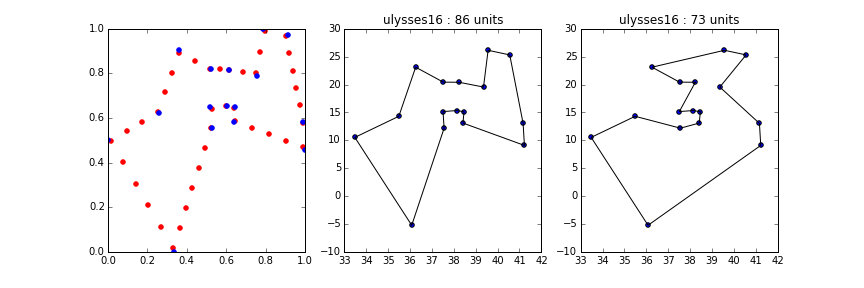
\includegraphics[scale=0.45]{figs/ulysses16}
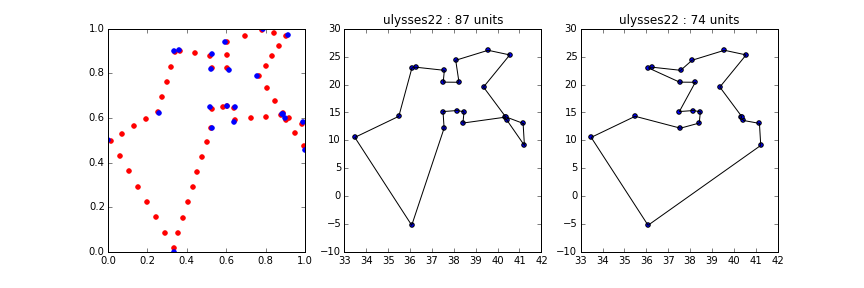
\includegraphics[scale=0.45]{figs/ulysses22}
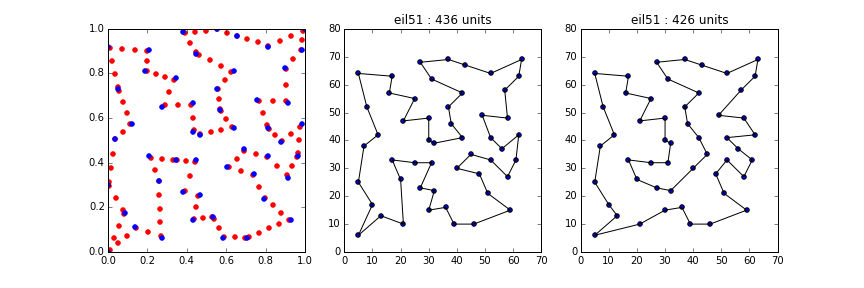
\includegraphics[scale=0.45]{figs/eil51}
 \end{center}
\end{figure}


\begin{figure}[!htb]
\begin{center}
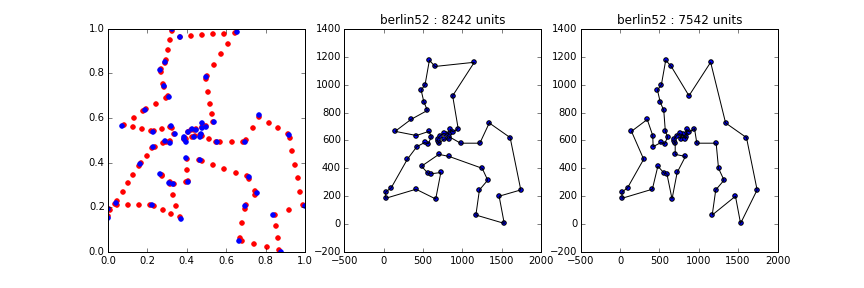
\includegraphics[scale=0.45]{figs/berlin52}
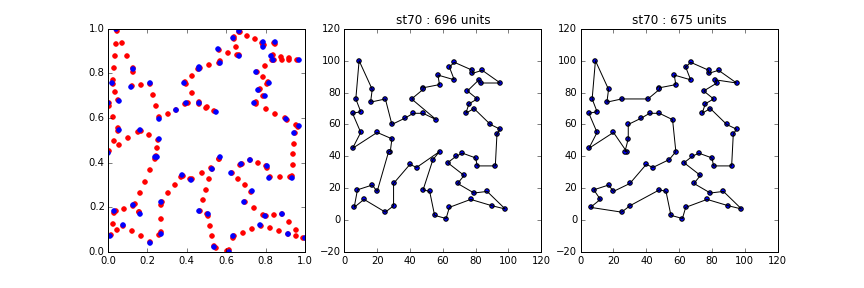
\includegraphics[scale=0.45]{figs/st70}
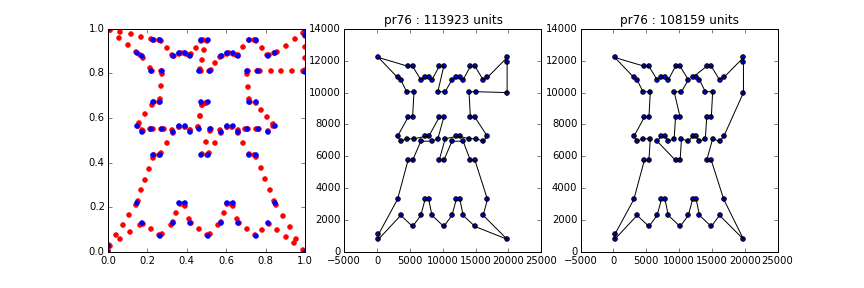
\includegraphics[scale=0.45]{figs/pr76}
 \end{center}
\end{figure}

 


\begin{figure}[!htb]
\begin{center}
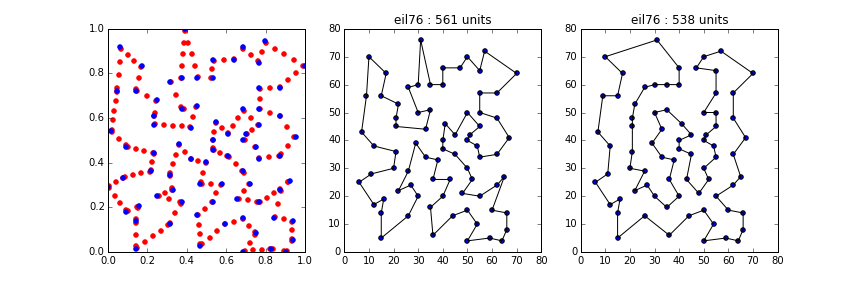
\includegraphics[scale=0.45]{figs/eil76}
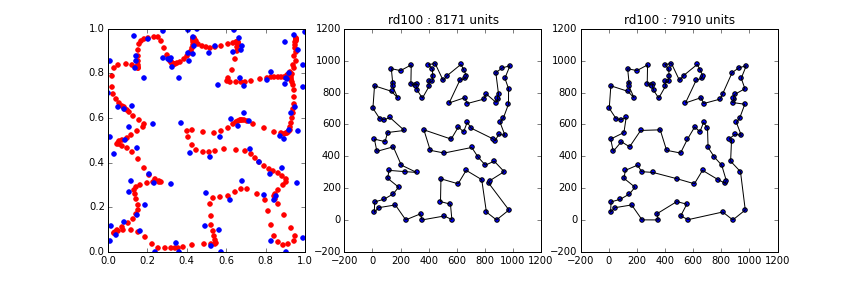
\includegraphics[scale=0.45]{figs/rd100}
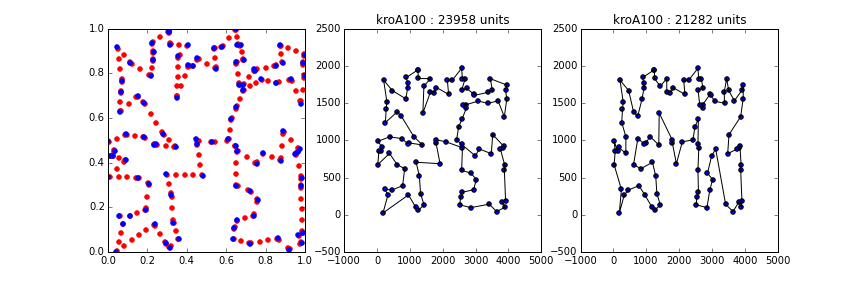
\includegraphics[scale=0.45]{figs/kroA100}

 \end{center}
\end{figure}


\begin{figure}[!htb]
\begin{center}
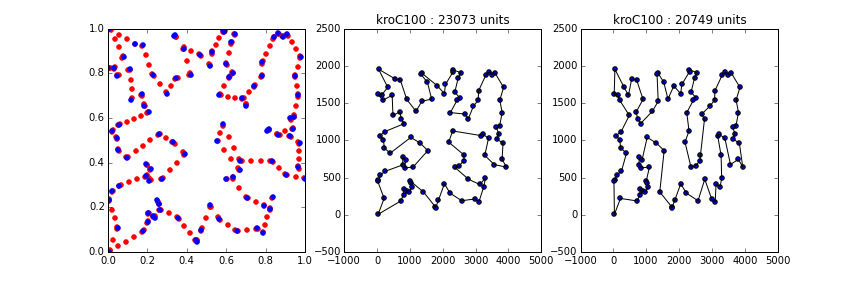
\includegraphics[scale=0.45]{figs/kroC100}
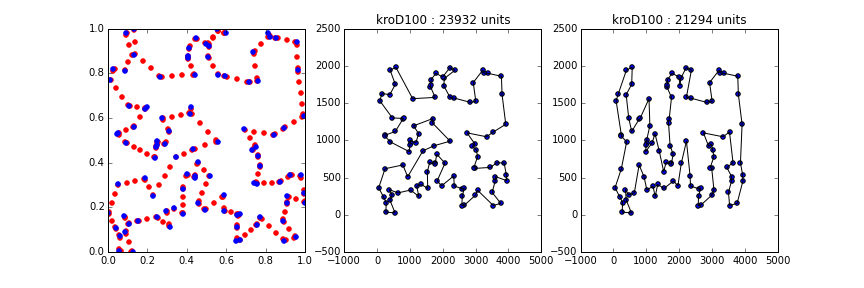
\includegraphics[scale=0.45]{figs/kroD100}
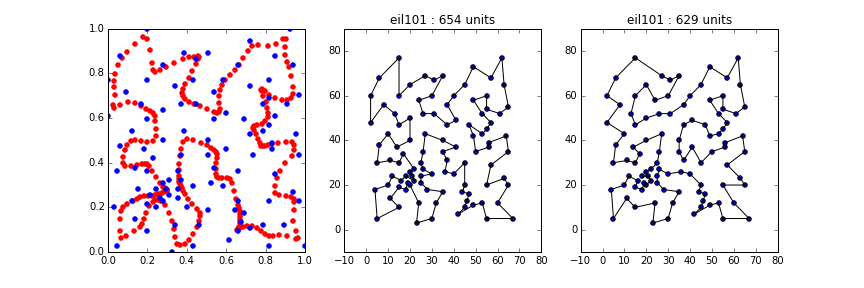
\includegraphics[scale=0.45]{figs/eil101}
 \end{center}
\end{figure}


\begin{figure}[!htb]
\begin{center}
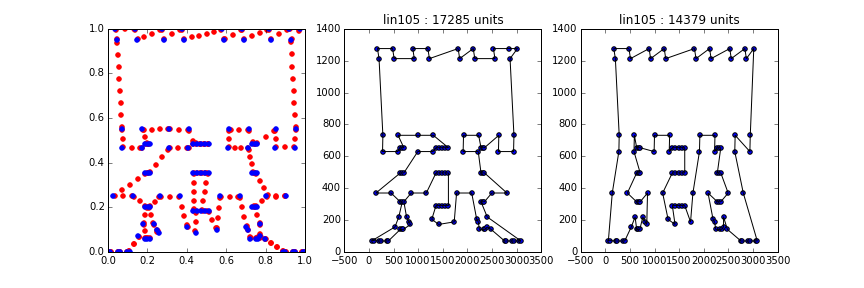
\includegraphics[scale=0.45]{figs/lin105}
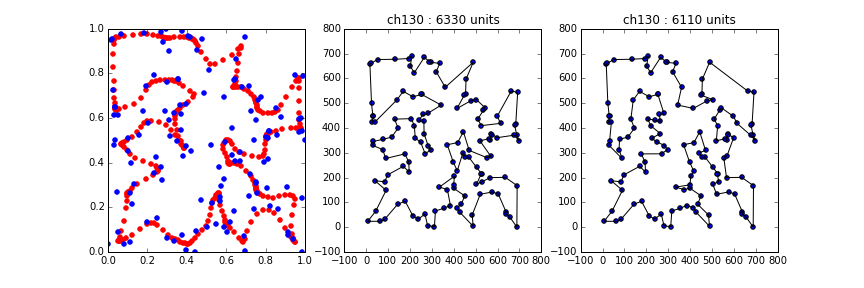
\includegraphics[scale=0.45]{figs/ch130}
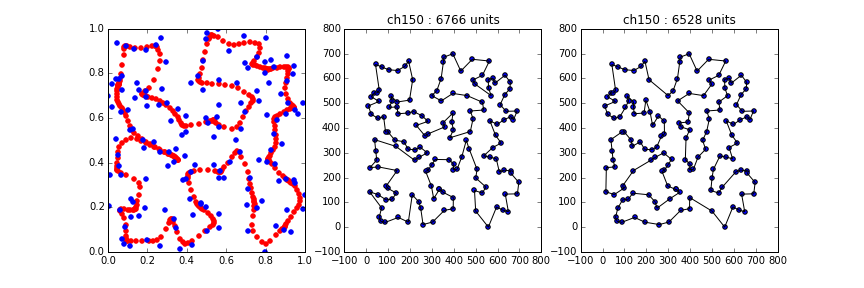
\includegraphics[scale=0.45]{figs/ch150}
 \end{center}
\end{figure}


 


\end{document}


